% !TEX root = ../latexnote.tex
\chapter{\LaTeX{} 基础}\label{chap:latex}
\section{\LaTeX{} 家族}\label{sec:latexfamily}
本节介绍一下各种名词,这里主要引用一篇知乎文章:\href{https://zhuanlan.zhihu.com/p/248669482}{TeX 家族(TeX, XeTeX, LuaTeX,XeLaTeX …看完这篇就懂了)},加之个人理解。
\elegantnewtheorem{explain}{}{defstyle}
\begin{explain*}{引擎}
    引擎是真正干活的程序。引擎的基本功能就是解释TeX语法,把字排成行,把行排成页,涉及到断字、断行、分页等算法。最原始的引擎是TeX。
    \begin{itemize}
        \item TeX:1978年由Donald Erwin Knuth(高德纳)开发。是后来大部分TeX相关的基础。其生成dvi文件,然后经由其他程序转换为pdf文件.
        \item pdfTeX:Tex语言的又一个实现,将TeX代码直接编译成PDF文件。
        \item XeTeX:TeX 语言的新的实现,支持 Unicode 编码和直接访问操作系统字体。
        \item LuaTeX:TeX 语言的一个完整的有扩展的实现。LuaTeX支持Unicode、系统字体和内嵌语言扩展,能直接输出PDF格式文件,也可以仍然输出 DVI 格式。
    \end{itemize}

    \bf{我的理解:TeX相当于汇编语言。}
\end{explain*}

\begin{explain*}[格式]
    TeX语言本身只有300个命令,晦涩难懂,只适合非正常的人类。一个简单的符号可能就需要多个命令来实现,可以将这些最基本的命令封装起来做个简写(宏)以实现特殊的目的。一堆简写的合集就构成了格式。格式可以与不同的引擎相结合。
    \begin{itemize}
        \item Plain TeX:由Don Knuth提供的最小的宏集合。
        \item LaTeX:更易于使用的宏集,最常见的一种格式。
        \item ConTeXt:另一种常见的格式。
    \end{itemize}


    \bf{我的理解:格式就是C语言等高级语言}
\end{explain*}

\begin{explain*}[编译命令]
    是实际调用的、结合了引擎和格式的命令。如 \lstinline{xelatex} 命令是结合  XeTeX 引擎和    LaTeX 格式的一个编译命令。
\end{explain*}

\begin{explain*}[宏包]
    一些辅助文件,在LaTeX中叫做packages,在ConTeXt中叫做modules。在LaTeX格式中,导言区的usepackage的作用就是引入各种宏包。宏包其实也是一堆基本的TeX命令的集合,只是其不够全,所以称之为宏包而不是格式。

    \bf{我的理解:宏包类似python的库,里面有封装好的函数}
\end{explain*}

\begin{explain*}[发行版]
    一个完整的TeX需要最基本的TeX引擎、格式支持、各种辅助宏包、一些转换程序、GUI、编辑器、文档查看器等等。通过选择不同的组合就构成了不同的发行版。
    \begin{itemize}
        \item TeX Live:支持Linux,Windows,Mac OS
        \item MiKTeX:只支持Windows
        \item CTeX:CTeX基于MiKTeX,并加入了中文的支持,只支持Windows。同时CTEX是一个网站,ctex是可以很好支持中文的宏包。
    \end{itemize}

    \bf{我的理解:IDE?}
\end{explain*}

\section{\LaTeX{} 安装}\label{sec:latexinstall}
参考\href{https://summersong.top/post/1f879cd9.html}{TexLive+VScode+SumatraPDF配置LaTex编辑环境}

\subsection{用户名为中文安装Texlive失败}\label{subsec:texlive_cn_username}
\qaq{问题:}在使用 GUI 界面安装时, 出现的错误形如图\ref{fig:failuregui}
\begin{figure}[!h]
    \centering
    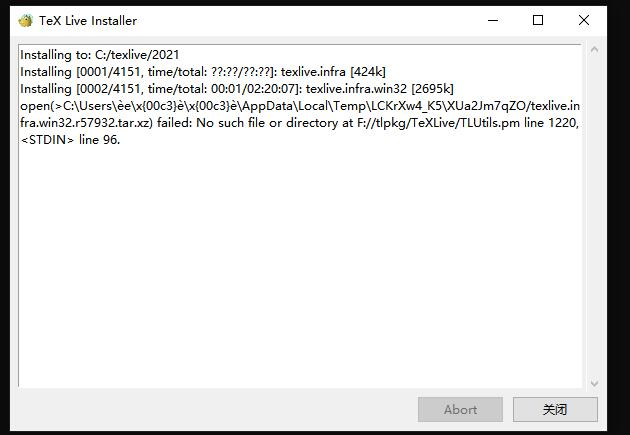
\includegraphics[width=0.8\textwidth]{figure/chap-basic/failuregui.jpg}
    \caption{Texlive 安装错误}\label{fig:failuregui}
\end{figure}

\qaq{解决方法:}参考\href{https://syvshc.github.io/2021-04-07-illegal-temp-cause-tlinstall-failure/}{Windows 不合法的缓存路径导致 TeX Live 安装失败},建议临时修改\lstinline{TEMP}与\lstinline{TMP}环境变量的值。在cmd中输入以下命令:
\begin{lstlisting}
    mkdir C:\temp
    set TEMP=C:\temp
    set TMP=C:\temp
\end{lstlisting}

然后运行安装脚本。

\section{\LaTeX{} 命令和代码结构}\label{sec:latexstructure}
\subsection{最短的\LaTeX{}代码}\label{subsec:shortlatexcode}
\begin{lstlisting}
\documentclass{article}
\begin{document}
Hello, \LaTeX{}!
\end{document}
\end{lstlisting}

上述代码是\LaTeX{} 排版的最短代码。下面简单介绍\LaTeX{}命令和代码的结构。

\subsection{\LaTeX{}命令和环境}\label{subsec:latexcommands}

\LaTeX{}命令以反斜杠 \hspace{0.2em}\textbackslash\hspace{0.2em} 开头,后面跟一串字母,如\lstinline{\LaTeX}。它们以任意非字母符号为界限。

要注意\LaTeX{} 命令是对大小写敏感的,比如输入 \lstinline{\LaTeX} 命令可以生成错落有致的 \LaTeX{} 字母组合,但输入 \lstinline{\Latex} 或者 \lstinline{\LaTex} 什么都得不到,还会报错;它们与 \lstinline{\LaTeX} 是不同的命令。

一些 \LaTeX{} 命令可以接收一些参数,参数的内容会影响命令的效果。\LaTeX{} 的参数分为可选参数和必选参数。可选参数以方括号 [] 包裹;必选参数一般以花括号 \{\} 包裹。还有些命令可以带一个星号*,带星号和不带星号的命令效果有一定差异,一般是带不带编号,比如章节标题。

\LaTeX{} 中还包括{\bf 环境},用以令一些效果在局部生效,或是生成特殊的文档元素。\LaTeX{} 环境的用法为一对命令 \lstinline{\begin} 和 \lstinline{\end}:
\begin{lstlisting}
\begin{环境名称}[可选参数]{必选参数}
    内容
\end{环境名称}
\end{lstlisting}

有些命令(如 \lstinline{\bfseries})会对其后所有内容产生作用。若要限制其作用范围,则需要使用{\bf 分组}。\LaTeX{} 使用一对花括号
\{\} 作为分组,在分组中使用的命令被限制在分组内,不会影响到分组外的内容。

\subsection{\LaTeX{}源代码结构}\label{subsec:latexsourcestructure}
LATEX 源代码以一个 \lstinline{\documentclass} 命令作为开头,它指定了文档使用的文档类。document 环境当中的内容是文档正文。

在 \lstinline{\documentclass} 和 \lstinline|\begin{document}|之间的位置称为{\bf 导言区}。在导言区中常会使用\lstinline{\usepackage} 命令调用{\bf 宏包},还会进行文档的全局设置。

\begin{lstlisting}

    \documentclass{...} % ...为某文档类,比如artile、book、report等
    % 导言区 
    \usepackage{ctex} %加载 ctex 宏包
    \begin{document}
    这里是正文。
    \end{document}
    %此后内容被忽略。

\end{lstlisting}

在正文区中,一般会包含一些文本、公式、图表、表格等内容。

\section{\LaTeX{} 文档类和宏包}\label{sec:latexclasses}
\subsection{\LaTeX{} 文档类}\label{subsec:latexdocclass}
文档类规定了 \LaTeX{} 源代码所要生成的文档的性质——普通文章、书籍、演示文稿、个人简历等等。\LaTeX{}源代码的开头须用\lstinline{\documentclass} 指定文档类:

\begin{lstlisting}
\documentclass[可选参数]{文档类名称}
\end{lstlisting}

文档类如\LaTeX{}提供的 article、report、book,在其基础上派生的一些文档类,如支持中文排版的 ctexart、ctexrep、ctexbook,或者有其它功能的一些文档类,如 moderncv、beamer 等。\LaTeX{} 提供的基础文档类见表\ref{tab:latex_doc_class},其中前三个习惯上称为“标准文档
类”。

\begin{table}[!h]
    \centering
    \caption{\LaTeX{} 文档类}
    \label{tab:latex_doc_class}
    \begin{tabular}{ll}
        \toprule
        类别      & 说明   \\
        \midrule
        article & 普通文章 \\
        book    & 书籍   \\
        report  & 报告   \\
        \hline
        letter  & 信件   \\
        slides  & 幻灯片  \\
        beamer  & 幻灯片  \\
        memoir  & 书籍类  \\
        acmart  & 科技论文 \\
        \bottomrule
    \end{tabular}
\end{table}

{\bf 可选参数}为文档类指定选项,以全局地规定一些排版的参数,如字号、纸张大小、单双面等等。比如调用 \lstinline{article} 文档类排版文章,指定纸张为 A4 大小,基本字号为 11pt,双面排版:
\begin{lstlisting}
\documentclass[11pt,a4paper,twoside]{article}
\end{lstlisting}

\subsection{\LaTeX{} 宏包}\label{subsec:latexpackage}
在使用 \LaTeX{} 时,时常需要依赖一些扩展来增强或补充\LaTeX{}的功能,比如排版复杂的表格、插入图片、增加颜色甚至超链接等等。这些扩展称为宏包。调用宏包的方法非常类似调用文档类的方法:
\begin{lstlisting}
\usepackage[可选参数]{宏包名称}
\end{lstlisting}
\lstinline{\usepackage} 可以一次性调用多个宏包:

\begin{lstlisting}
    % 一次性调用三个排版表格常用的宏包
    \usepackage{tabularx, makecell, multirow}
\end{lstlisting}

\section{\LaTeX{} 使用到的文件类型}\label{sec:latexfiletypes}

除了源代码文件 \lstinline{.tex} 以外,我们在使用 \LaTeX{} 时还可能接触到各种格式的文件。本节简单介绍一下在使用 \LaTeX{} 时能够经常见到的文件。

每个宏包和文档类都是带特定扩展名的文件,除此之外也有一些文件出现于 \LaTeX{} 模板中:

\begin{itemize}
    \item \lstinline{.sty} 宏包文件。宏包的名称与文件名一致。
    \item \lstinline{.cls} 文档类文件。文档类名称与文件名一致。
    \item \lstinline{.bib} BibTeX 参考文献数据库文件。
    \item \lstinline{.bst} BibTeX 用到的参考文献格式模板。
\end{itemize}

\LaTeX{} 在编译过程中除了生成 .dvi 或 .pdf 格式的文档外,还可能会生成相当多的辅助文件和日志。一些功能如交叉引用、参考文献、目录、索引等,需要先通过编译生成辅助文件,然后再次编译时读入辅助文件得到正确的结果,所以复杂的 \LaTeX{} 源代码可能要编译多次:

\begin{itemize}
    \item \lstinline{.log} 排版引擎生成的日志文件,供排查错误使用。
    \item \lstinline{.aux} \LaTeX{} 生成的主辅助文件,记录交叉引用、目录、参考文献的引用等。
    \item \lstinline{.toc} \LaTeX{} 生成的目录记录文件。
    \item \lstinline{.lof} \LaTeX{} 生成的图片目录记录文件。
    \item \lstinline{.lot} \LaTeX{} 生成的表格目录记录文件。
    \item \lstinline{.bbl} BibTeX 生成的参考文献记录文件。
    \item \lstinline{.blg} BibTeX 生成的日志文件。
    \item \lstinline{.idx} \LaTeX{} 生成的供 makeindex 处理的索引记录文件。
    \item \lstinline{.ind} makeindex 处理 .idx 生成的用于排版的格式化索引文件。
    \item \lstinline{.ilg} makeindex 生成的日志文件。
    \item \lstinline{.out} hyperref 宏包生成的 PDF 书签记录文件。
\end{itemize}

\section{\LaTeX{} 文件组织方式}\label{sec:latexfileorganization}

编写长篇文档时,例如当编写书籍、毕业论文时,单个源文件会使修改、校对变得十分困难。将源文件分割成若干个文件,例如将每章内容单独写在一个文件中,会大大简化修改和校对的工作。

\LaTeX{} 提供了命令 \lstinline{\include} 用来在源代码里插入文件:

\begin{lstlisting}
\include{chapter1}
\include{chapter2}
\include{chapter3}
\end{lstlisting}

需要注意的是,\lstinline{\include} 命令在读入新的文件之前会另起一页。有的时候我们不需要这样,则用\lstinline{\input} 命令,它仅仅只是将文件里面的内容插入到当前位置。

当导言区内容较多时,常常将其单独放置在一个 \lstinline{.tex} 文件中,再用 \lstinline{\input} 命令插入。复杂的图、表、代码等也会用类似的手段处理。

LATEX 还提供了一个 \lstinline{\includeonly} 命令来组织文件,用于导言区,指定只载入某些文件。导言区使用了 \lstinline{\includeonly} 后,正文中不在其列表范围的 \lstinline{\include}命令不会起效:
\begin{lstlisting}
\includeonly{chapter1,chapter3}
\end{lstlisting}

